\subsection{T2: Matrix-Level Structural Methods}
\label{sec:t2}

\subsubsection{Family Overview and Meta-Pipeline Position}
\label{sec:t2-overview}

T2 contains optimizers whose primary operation uses the matrix structure of
Transformer parameters.  T1 methods flatten a weight tensor and treat it as a
collection of independent coordinates.  T2 methods instead work directly at the
matrix level, coupling rows, columns, singular directions, Kronecker factors,
or low-rank subspaces.
The typical object is a two-dimensional weight matrix
$W_t\in\mathbb{R}^{m\times n}$ with stochastic gradient
$G_t\in\mathbb{R}^{m\times n}$.  The family is therefore tied to parameter
topology.  Attention projections, MLP projections, and other dense matrix
weights are natural targets, whereas biases, normalization parameters,
embeddings, and sometimes output heads fall back to an element-wise optimizer
such as AdamW or SGD.  This matrix routing is the S1 (parameter scoping and
routing) stage of the meta-pipeline, and by deciding which parameters are
treated as matrices it determines whether matrix transforms such as
orthogonalization or Kronecker-factored preconditioning can be applied at all.

\begin{figure*}[t]
  \centering
  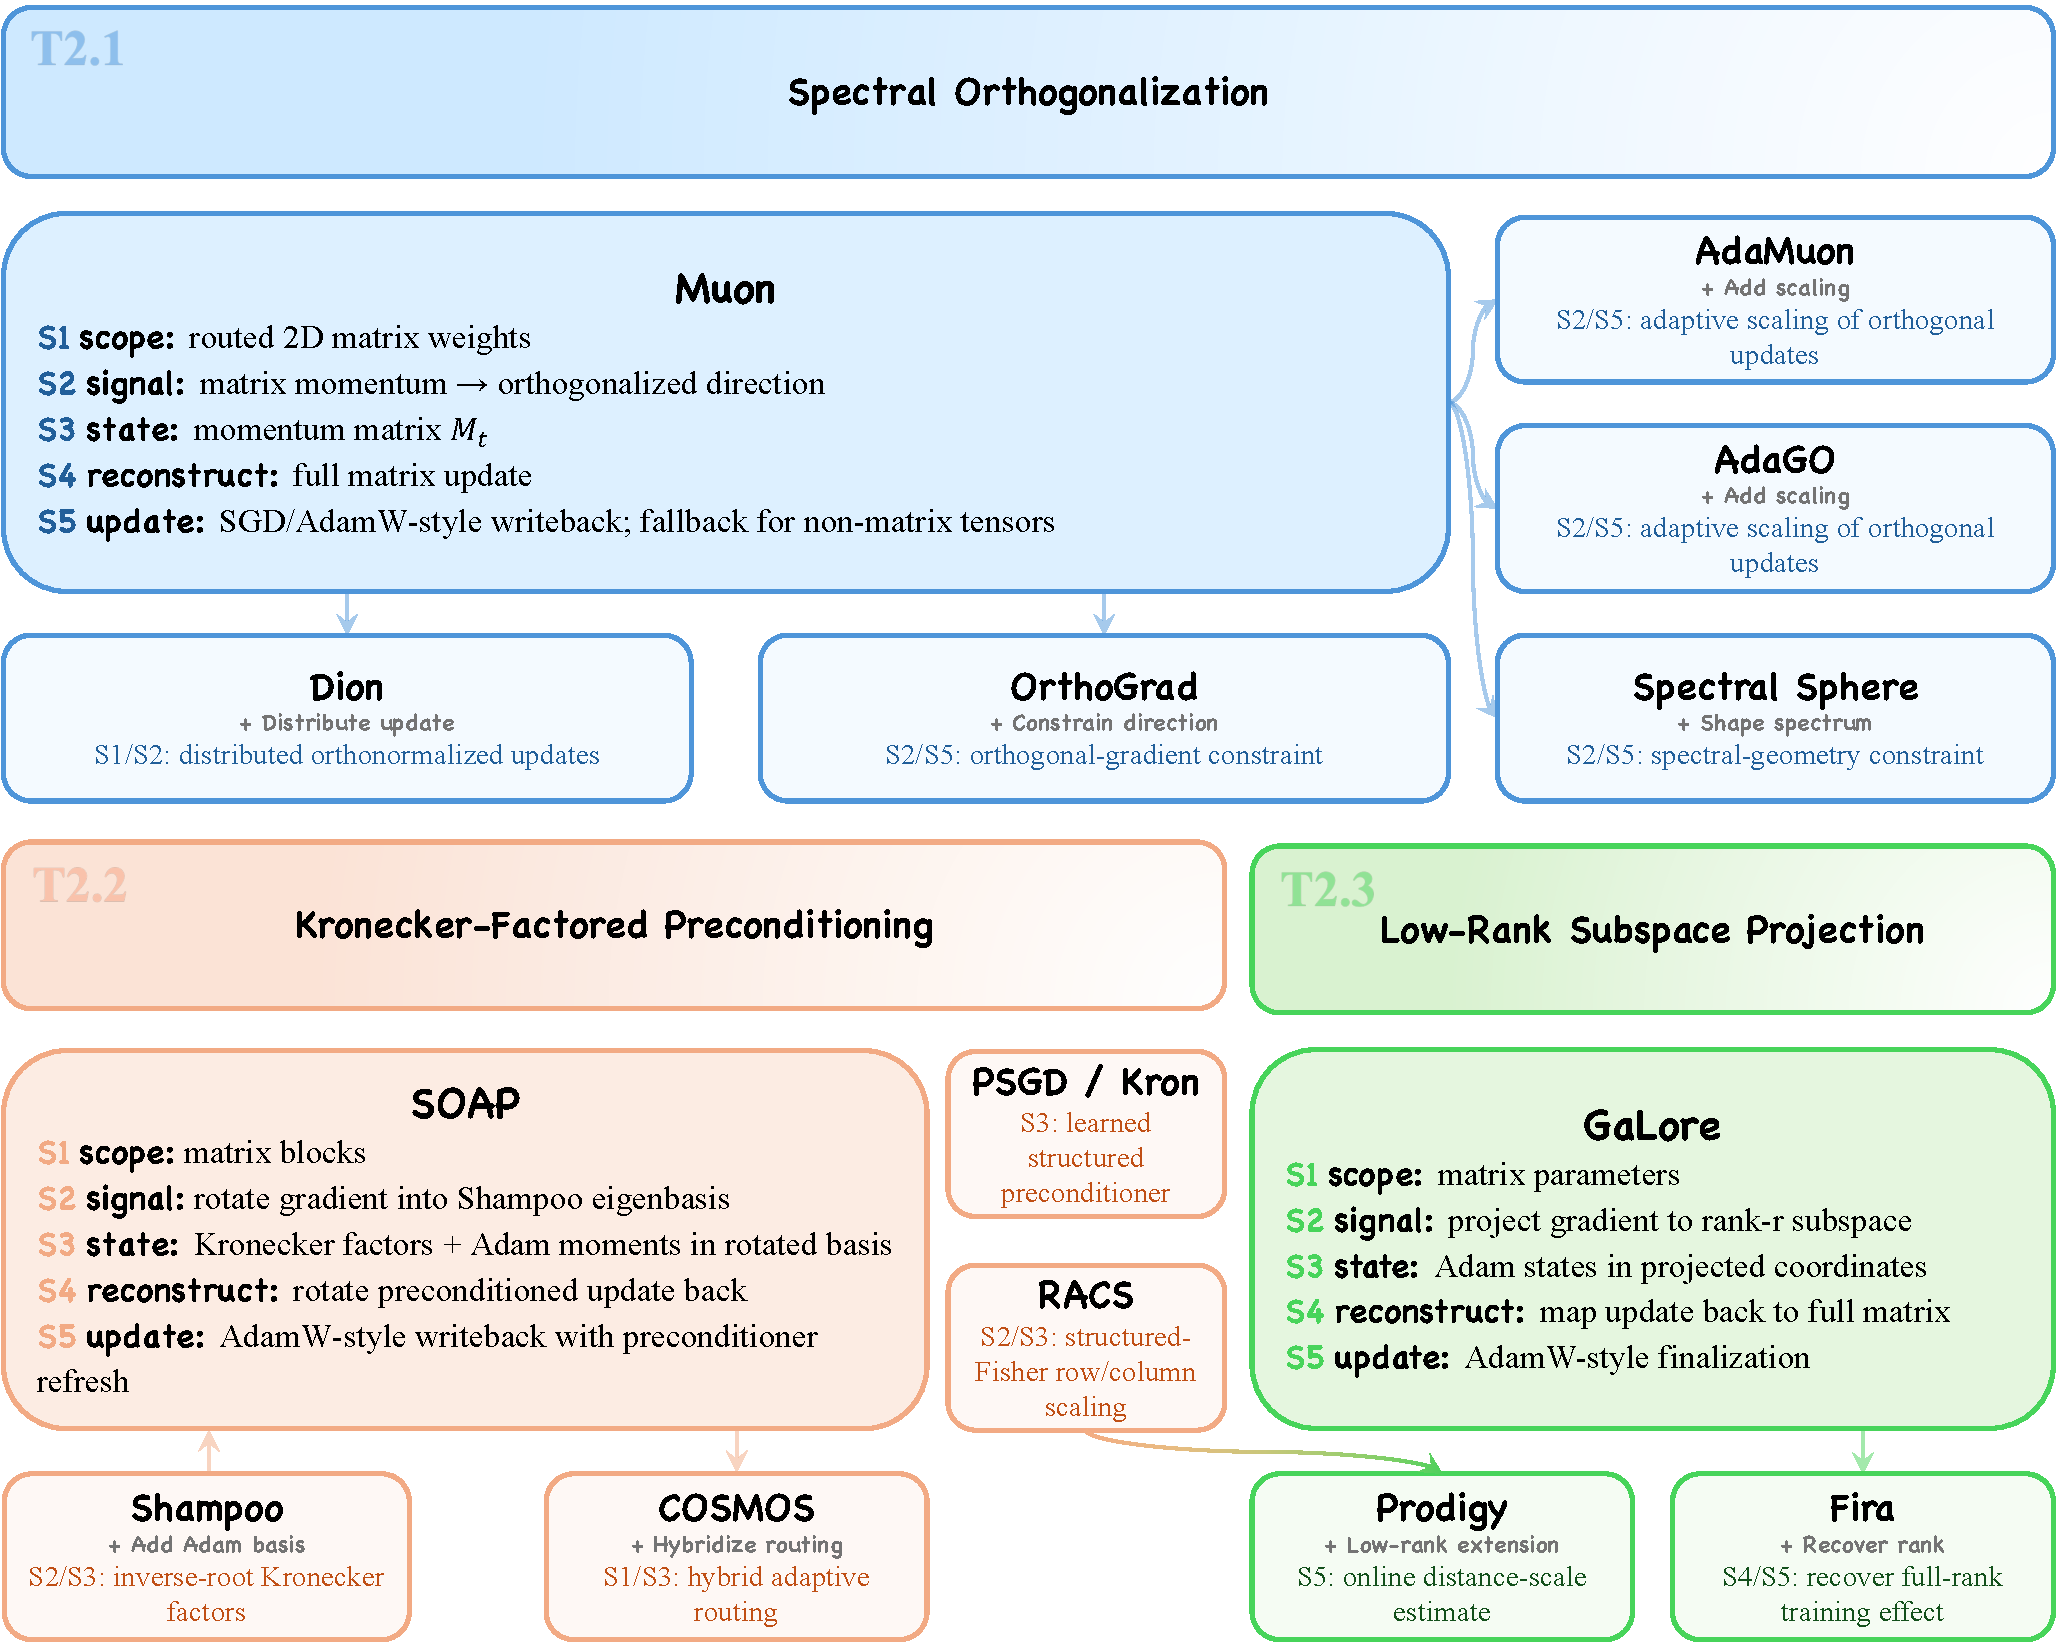
\includegraphics[width=0.75\textwidth]{figures/opt_t2.pdf}
  \caption{Mechanism schematic for T2 matrix-level structural methods.  The
  schematic summarizes the three matrix routes used in this survey: spectral
  direction selection, Kronecker or structured-Fisher preconditioning, and
  low-rank subspace projection.  It is a taxonomy guide rather than an
  empirical ranking.}
  \label{fig:t2_family_mechanism}
\end{figure*}

\paragraph{Subclass structure and membership.}
Figure~\ref{tab:t2_family_taxonomy} gives the subclass-level optimizer list for T2, and the
three subclasses below specify the corresponding optimizer membership.  The
split is based on the primary matrix operation: spectral direction selection,
structured matrix preconditioning, or subspace projection.
\begin{enumerate}[label=\textbf{T2.\arabic*},leftmargin=*,itemsep=2pt]
  \item \textbf{Spectral orthogonalization.}
  This subclass contains Muon, RMNP~\cite{deng2026rmnp}, MOGA, Dion, AdaMuon, OrthoGrad, AdaGO,
  and Spectral Sphere.  Its members construct an orthogonalized or spectral-geometry update
  from a two-dimensional gradient or momentum object, with Muon as the
  subclass's central representative method for LLMs~\citep{jordan2024muon,pethick2025normlmo,sfyraki2025lions}.
  \item \textbf{Kronecker-factored preconditioning.}
  This subclass contains SOAP, Shampoo, MARS-Shampoo, COSMOS, Kron, PSGD,
  SPlus, and RACS.  Its members estimate row/column curvature, covariance, structured Fisher
  factors, or learned Kronecker-style preconditioners, with Shampoo and SOAP as
  the subclass's core representative methods, around which its mathematical
  framework is built~\citep{gupta2018shampoo,vyas2025soap}.
  \item \textbf{Low-rank subspace projection.}
  This subclass contains GaLore, Fira, and Alice.  Its members project the
  gradient and optimizer state into a low-dimensional subspace, update there,
  and reconstruct a full matrix update, with GaLore as the canonical LLM
  example~\citep{zhao2024galore}.
\end{enumerate}

At the family level, a matrix-structured update can be summarized as
\begin{equation}
  Z_t = B_t^\top G_t C_t,\quad
  \widetilde{\Delta}_t = \Phi_t(Z_t;\mathcal{S}_{t-1}),\quad
  \Delta_t = A_t\widetilde{\Delta}_t D_t^\top,
  \label{eq:t2-matrix-template}
\end{equation}
where $B_t,C_t$ are the left and right analysis bases that rotate or project
the gradient into a new coordinate system, $\Phi_t$ is the direction or
preconditioning rule applied in that coordinate system, $\mathcal{S}_{t-1}$
denotes the structured state, and $A_t,D_t$ map the transformed update back to
the parameter matrix.  Muon uses an SVD or polar basis and flattens the
singular values.  Shampoo and SOAP use Kronecker or Fisher eigenbases.  GaLore
uses projection and reconstruction maps with rank $r\ll\min(m,n)$.  This
template is intentionally broader than any one algorithm.  Its role is to make clear
that T2 changes the geometry in which a matrix update is analyzed before the
usual optimizer writeback is applied.

% Auto-generated by code/generate_taxonomy_figures.py; do not edit by hand.
% \begin{table*}[!htbp]
%   \centering
%   \caption{Taxonomy of matrix-level structural optimizers.}
%   \label{tab:t2_family_taxonomy}
%   \scriptsize
%   \setlength{\tabcolsep}{4pt}
%   \renewcommand{\arraystretch}{1.16}
%   \arrayrulecolor{optHiddenBlack}
%   \begin{tabularx}{0.92\textwidth}{@{}>{\raggedright\arraybackslash}p{0.25\textwidth}>{\raggedright\arraybackslash}X@{}}
%     \hline
%     \textbf{Subclass} & \textbf{Optimizers} \\
%     \hline
%     \textbf{\textit{T2.1: Spectral Orthogonalization}} & Muon~\cite{jordan2024muon,pethick2025normlmo}, RMNP~\cite{deng2026rmnp}, MOGA~\cite{xu2026width}, Dion~\cite{ahn2025dion}, AdaMuon~\cite{si2025adamuon}, OrthoGrad~\cite{hedges2025orthograd}, AdaGO~\cite{zhang2025adagrad}, Spectral Sphere~\cite{xie2026controlled} \\
%     \hline
%     \textbf{\textit{T2.2: Kronecker-Factored Preconditioning}} & SOAP~\cite{vyas2025soap}, Shampoo~\cite{gupta2018shampoo}, MARS-Shampoo~\cite{yuan2024mars,gupta2018shampoo}, COSMOS~\cite{liu2025cosmos}, Kron~\cite{li2017preconditioned}, PSGD~\cite{li2017preconditioned,li2022black}, SPlus~\cite{frans2026stable}, RACS~\cite{gong2025towards} \\
%     \hline
%     \textbf{\textit{T2.3: Low-Rank Subspace Projection}} & GaLore~\cite{zhao2024galore}, Fira~\cite{chen2026fira}, Alice~\cite{gong2025towards} \\
%     \hline
%   \end{tabularx}
% \end{table*}

\definecolor{hidden-blue}{HTML}{4a90e2}
\definecolor{hidden-black}{HTML}{333333}
\tikzstyle{my-box}=[
  rectangle,
  draw=hidden-black,
  rounded corners,
  text opacity=1,
  minimum height=1.5em,
  minimum width=5em,
  inner sep=2pt,
  align=center,
  fill opacity=.5,
]
\tikzstyle{root}=[
  align=center,
]
\tikzstyle{leaf}=[
  my-box,
  minimum height=1.5em,
  text=black,
  font=\normalsize,
  inner xsep=5pt,
  inner ysep=4pt,
  text width=10.5em,
  fill opacity=1,
]
\tikzstyle{leaf1}=[
  my-box,
  minimum height=1.5em,
  fill=yellow!32,
  text=black,
  font=\normalsize,
  inner xsep=5pt,
  inner ysep=4pt,
  text width=17em,
  align=left,
]
\tikzstyle{leaf2}=[
  my-box,
  minimum height=1.5em,
  fill=hidden-blue!57,
  text=black,
  font=\normalsize,
  inner xsep=5pt,
  inner ysep=4pt,
  text width=17em,
  align=left,
]
\tikzstyle{leaf3}=[
  my-box,
  minimum height=1.5em,
  fill=purple!27,
  text=black,
  font=\normalsize,
  inner xsep=5pt,
  inner ysep=4pt,
  text width=17em,
  align=left,
]

\begin{figure*}[!htbp]
\centering
\resizebox{\textwidth}{!}{
\begin{forest}
forked edges,
for tree={
grow=east,
reversed=true,
anchor=base west,
parent anchor=east,
child anchor=west,
base=left,
font=\large,
rectangle,
draw=hidden-black,
rounded corners,
align=left,
minimum width=4em,
edge+={darkgray, line width=1pt},
s sep=4pt,
inner xsep=5pt,
inner ysep=4pt,
line width=1.1pt,
ver/.style={rotate=90, child anchor=north, parent anchor=south, anchor=center},
},
where level=1{text width=11em, font=\normalsize}{},
where level=2{text width=34.5em, tier=citations, font=\small}{},
[
    T2-based Optimizers,
    ver, fill=brown!10!white, text=hidden-black, root
    [
        T2.1: Spectral Orthogonalization,
        fill=yellow!32, leaf1
        [{
            Muon~\cite{jordan2024muon,pethick2025normlmo},
            RMNP~\cite{deng2026rmnp},
            MOGA~\cite{xu2026width},
            Dion~\cite{ahn2025dion},
            AdaMuon~\cite{si2025adamuon},
            OrthoGrad~\cite{hedges2025orthograd}, \\
            AdaGO~\cite{zhang2025adagrad},
            Spectral Sphere~\cite{xie2026controlled}
        }, fill=yellow!12]
    ]
    [
        T2.2: Kronecker-Factored \\ Preconditioning,
        fill=hidden-blue!57, leaf2
        [{
            SOAP~\cite{vyas2025soap},
            Shampoo~\cite{gupta2018shampoo},
            MARS-Shampoo~\cite{yuan2024mars,gupta2018shampoo},
            COSMOS~\cite{liu2025cosmos},
            Kron~\cite{li2017preconditioned}, \\
            PSGD~\cite{li2017preconditioned,li2022black},
            SPlus~\cite{frans2026stable},
            RACS~\cite{gong2025towards}
        }, fill=hidden-blue!15]
    ]
    [
        T2.3: Low-Rank Subspace Projection,
        fill=purple!27, leaf3
        [{
            GaLore~\cite{zhao2024galore},
            Fira~\cite{chen2026fira},
            Alice~\cite{gong2025towards}
        }, fill=purple!12]
    ]
  ]
\end{forest}
}
\caption{Taxonomy of matrix-level structural optimizers.}
\label{tab:t2_family_taxonomy}
\end{figure*}


Together, these subclasses make T2 the family where S1 routing, S2
transformation, S3 structured state, and S4 reconstruction all become
first-class design choices.  S5 is usually less distinctive: many T2 methods
still use SGD-style or AdamW-style final writeback after the matrix transform,
possibly with decoupled weight decay, damping, or method-specific scaling.

This definition also fixes the boundary with neighboring families.  Whether a
method belongs to T2 depends on whether its update rule genuinely uses the
matrix geometry.  Conversely, whether a method belongs to T4 likewise depends
on its mechanism.  GaLore does reduce optimizer-state memory, but it does so by
changing the mathematical subspace in which the gradient and Adam state live,
so its primary mechanism is T2.3 (low-rank subspace), and state compression is
only an effect of that choice.  If an additional contribution directly
quantizes, shards, shares, or frees optimizer state, that contribution should
be recorded as a secondary T4 tag.  Likewise,
sharpness-aware wrappers, layer-wise trust ratios, or post-update filters
remain T5 unless the matrix transform itself is the primary new operation.

\subsubsection{LMO-Driven Four-Axis Interpretation}
\label{sec:t2-lmo-four-axis}

The four-axis view in Section~\ref{sec:lmo-four-axis} is especially useful for
T2 because it separates the basis used to analyze a matrix update from the
state used to estimate its scale.  A generic T2 coordinate can be written as
\begin{equation}
  \big((B_t,C_t),\ \psi_t,\ \hat{H}_t,\ \alpha,\ \widehat{G}_t,\ \mathcal{S}_t\big),
\end{equation}
where $B_t$ and $C_t$ are left and right analysis bases, $\psi_t$ is the
matrix direction map, $\hat{H}_t$ is a structured curvature or covariance
proxy when present, and $\mathcal{S}_t$ records whether the optimizer state is
full-rank, factored, or projected.  In T1, $B_t=C_t=I$ and $\mathcal{S}_t$ is
usually full coordinate state.  In T2, the basis itself is part of the method.

For Muon-style spectral-normalization methods, the defining map is a polar or
orthogonalized direction.  With momentum matrix
$M_t=\beta M_{t-1}+(1-\beta)G_t$ and singular value decomposition
$M_t=U_t\Sigma_tV_t^\top$, the update is
\begin{equation}
  W_{t+1}=W_t-\eta_t\,U_tV_t^\top ,
  \label{eq:t2-muon-polar}
\end{equation}
where $U_tV_t^\top$ is usually approximated by a few Newton--Schulz matrix
multiplications rather than an explicit SVD.  This direction is the full polar
factor, so it keeps the singular vectors while flattening every singular value
to one.

Axis~III holds this direction in both the LMO and the preconditioner readings
(Table~\ref{tab:four-axis-instantiation}), and the two agree on the same
$U_tV_t^\top$.  From the LMO side, it is the steepest matrix direction on the
spectral-norm ball,
\begin{equation}
  U_tV_t^\top = \argmax_{\|X\|_{S_\infty}\le 1}\ \langle M_t,X\rangle,
\end{equation}
where $\|\cdot\|_{S_\infty}$ is the spectral norm and
$\langle M_t,X\rangle=\operatorname{tr}(M_t^\top X)$.  By the von Neumann trace
inequality $\langle M_t,X\rangle\le\sum_i\sigma_i(M_t)\sigma_i(X)\le\sum_i\sigma_i(M_t)$,
with equality at $X=U_tV_t^\top$, the steepest direction is exactly the polar
factor.  From the preconditioner side, the same direction is a Gram
preconditioning of the momentum,
\begin{equation}
  \operatorname{msign}(M_t)=(M_tM_t^\top)^{-1/2}M_t=U_tV_t^\top ,
\end{equation}
where $\operatorname{msign}(\cdot)$ is the matrix sign function that sets all
singular values to one, matching the Axis~III metric $H_t=M_tM_t^\top$ in
Table~\ref{tab:four-axis-instantiation}.  The two readings are the two faces of
the same operator $\Phi_t$, and they differ only in whether the geometry is
charged to the direction map $\psi_t$ or to the metric $H_t$.

Kronecker-factored preconditioning occupies a different point in the same
matrix space.  For Shampoo, the matrix case maintains row and column factors
\begin{equation}
  L_t=\beta L_{t-1}+(1-\beta)G_tG_t^\top,\quad
  R_t=\beta R_{t-1}+(1-\beta)G_t^\top G_t,
  \label{eq:t2-shampoo-factors}
\end{equation}
and applies an inverse-root preconditioner,
\begin{equation}
  \Delta_t = L_t^{-1/4}G_tR_t^{-1/4},\quad W_{t+1}=W_t-\eta_t\Delta_t .
  \label{eq:t2-shampoo-update}
\end{equation}
As with Muon, Axis~III holds this update in both the LMO and the preconditioner
readings (Table~\ref{tab:four-axis-instantiation}).  From the preconditioner
side, the row and column factors combine into a Kronecker metric
\begin{equation}
  H_t = L_t^{1/4}\otimes R_t^{1/4},\quad
  \operatorname{vec}(\Delta_t)=H_t^{-1}\operatorname{vec}(G_t),
\end{equation}
whose analysis basis is the eigenbasis of $L_t$ and $R_t$.  The curvature proxy
is a Kronecker-structured matrix that captures coordinate coupling and is richer
than the diagonal vector of Adam.  From the LMO side, the same direction is the
steepest matrix direction on the Kronecker-metric ball
$\{X:\|L_t^{1/4}XR_t^{1/4}\|_F\le\rho\}$, an ellipsoid (Mahalanobis ball)
stretched and rotated by that metric, so Shampoo returns a continuous
preconditioned gradient.
SOAP keeps this basis idea but runs Adam-style coordinate adaptation after
rotating the gradient into the Shampoo eigenbasis, then rotates the update
back~\citep{vyas2025soap}.  It is therefore a bridge between T1 and T2, with a
coordinate-wise adaptive denominator whose coordinates have shifted from raw
parameters to learned matrix-curvature coordinates.

Low-rank projection methods move along Axis~I
(Table~\ref{tab:four-axis-instantiation}), placing the whole update in a
low-dimensional subspace while the curvature estimate largely follows Adam.
GaLore is the representative example, choosing or refreshing a projection basis
$P_t\in\mathbb{R}^{m\times r}$ with $r\ll\min(m,n)$ and projecting the gradient,
\begin{equation}
  \widetilde{G}_t=P_t^\top G_t,
  \label{eq:t2-galore-project}
\end{equation}
running Adam or AdamW state evolution on $\widetilde{G}_t$, and reconstructing a
full update by $\Delta_t=P_t\widetilde{\Delta}_t$.  Because the optimizer state
lives only in the projected low-dimensional coordinates, memory drops
accordingly.  The risk is approximation error.  Useful high-rank gradient
components may be removed unless the basis refresh, rank allocation, or residual
pathway captures them.

\subsubsection{Representative Methods}
\label{sec:t2-methods}

The following discussion follows the T2.1--T2.3 subclass order introduced
above.  Within each subclass, representative methods are grouped by the local
matrix operation they modify rather than by chronology.

\paragraph{Spectral Orthogonalization.}
\label{sec:t2-spectral}

The spectral branch asks whether a matrix update should preserve the
singular-vector frame but discard the singular-value scale.  At the survey
level, its core operation is
\begin{equation}
  M_t=\beta M_{t-1}+(1-\beta)G_t,\quad
  D_t=\operatorname{Polar}(M_t)
      = U_tV_t^\top
      \approx \operatorname{NS}_K(M_t),
  \label{eq:t2-spectral-template}
\end{equation}
where $M_t=U_t\Sigma_tV_t^\top$ and $\operatorname{NS}_K$ denotes a finite
Newton--Schulz approximation to the polar factor.  The resulting update is
usually $W_{t+1}=W_t-\eta_tD_t$ on routed matrix parameters.
\begin{itemize}
  \setlength{\itemsep}{2pt}
  \item \textbf{Canonical orthogonalized-update line.}  Muon is the central
  T2.1 method because it turns the matrix momentum into an orthogonalized
  update rather than a coordinate-wise adaptive update.  In practical LLM
  implementations, Muon is usually applied only to selected two-dimensional
  hidden-layer weights, while embeddings, scalar parameters, normalization
  parameters, and other excluded tensors use an SGD or AdamW-style fallback
  route~\citep{jordan2024muon}.
  \item \textbf{Routing and scaling extensions.}  Dion proposes distributed
  orthonormalized updates and broader parameter handling, making the S1
  routing and systems pathway more explicit~\citep{ahn2025dion}.  AdaMuon and
  AdaGO add adaptive scaling logic to orthogonalized updates, placing them at
  the boundary between T2.1 direction selection and T1-style step-size
  adaptation~\citep{si2025adamuon,zhang2025adagrad}.
  \item \textbf{Spectral-geometry boundary methods.}  OrthoGrad and Spectral
  Sphere are useful boundary points rather than central LLM optimizer
  baselines: the former studies orthogonal-gradient constraints for
  calibration, while the latter studies controlled LLM training under
  spectral-sphere geometry~\citep{hedges2025orthograd,xie2026controlled}.
\end{itemize}

The common thread is a single direction choice, namely to preserve the
singular-vector frame and flatten the singular spectrum.  Whether it
consistently beats AdamW, Shampoo, or SOAP depends on the setting.  The open
empirical question is whether the spectral direction remains beneficial after
matching batch size, warmup, weight decay, fallback optimizer, matrix-only
scope, step time, and tuning budget.  Recent mechanism and fine-tuning studies already warn that
Muon-style conclusions can be protocol-sensitive
~\citep{qu2026muonfinetune,shumaylov2026muonnot}.

\paragraph{Kronecker-Factored Preconditioning.}
\label{sec:t2-kronecker}

The Kronecker branch asks whether a matrix update should be scaled in row and
column curvature coordinates or kept in raw parameter coordinates.  The shared
template is
\begin{align}
  L_t &= \beta L_{t-1}+(1-\beta)G_tG_t^\top,\quad
  R_t = \beta R_{t-1}+(1-\beta)G_t^\top G_t, \\
  \bar{G}_t &= P_{L,t}^\top G_t P_{R,t},\quad
  \Delta_t = P_{L,t}\,\Psi_t(\bar{G}_t;\mathcal{S}_t)\,P_{R,t}^\top,
  \label{eq:t2-kronecker-adaptive-template}
\end{align}
where $P_{L,t}$ and $P_{R,t}$ are eigenvectors or structured bases derived
from row/column statistics.  Shampoo instantiates $\Psi_t$ as inverse-root
preconditioning, whereas SOAP uses Adam-style coordinate adaptation in this
rotated basis.
\begin{itemize}
  \setlength{\itemsep}{2pt}
  \item \textbf{Inverse-root preconditioning base.}  Shampoo is the
  mathematical base of T2.2.  It stores per-mode row and column statistics and
  applies matrix inverse roots~\citep{gupta2018shampoo}, approximating the full
  $(mn)\times(mn)$ curvature matrix with two small factors while keeping more
  coordinate coupling than Adam's per-coordinate diagonal second moment.  For
  matrices, this yields the factors and update in
  Eqs.~\eqref{eq:t2-shampoo-factors}--\eqref{eq:t2-shampoo-update}.
  The benefit is a structured approximation to second-order information; the
  cost is nontrivial state, matrix-root computation, numerical damping, and a
  refresh schedule for the preconditioners.
  \item \textbf{Adam-in-eigenbasis and practical routing.}  SOAP updates the
  Shampoo line by adding Adam-like adaptation in the Shampoo eigenbasis
  ~\citep{vyas2025soap}.  Conceptually, it first chooses the matrix basis from
  Kronecker factors and then applies diagonal adaptivity in that rotated
  coordinate system.  COSMOS extends the practical branch by combining hybrid
  adaptive routing with memory-efficient LLM training goals
  ~\citep{liu2025cosmos}.
  \item \textbf{Learned and structured-Fisher preconditioners.}  PSGD and
  Kron-like instances form a broader learned-preconditioner branch.  The early
  PSGD formulation and later Lie-group preconditioner view learn structured
  preconditioners rather than using Shampoo's fixed inverse-root construction
  ~\citep{li2017preconditioned,li2022black}.  RACS is placed in T2.2 because its
  row-and-column scaled SGD is based on a structured Fisher approximation,
  whereas the low-rank extension in the same source is represented by
  Alice~\citep{gong2025towards}.
\end{itemize}

The common thread is structured matrix scaling.  T2.2 differs from T2.1
because it uses magnitude information in row/column or Fisher coordinates
rather than only flattening a spectrum.  It differs from T2.3 because it does
not make low-rank projection the primary state space.  Because Shampoo and SOAP
tend to improve loss per token while paying a high per-step cost, benchmark
claims for this subclass should report loss at a fixed token budget alongside
loss normalized by wall-clock or step time, so that the per-step overhead is
counted, together with the preconditioner refresh frequency, damping, and
memory overhead that drive this cost.

\paragraph{Low-Rank Subspace Projection.}
\label{sec:t2-low-rank}

The low-rank branch asks whether the optimizer state should live in a
projected matrix subspace.  Its survey-level template is
\begin{equation}
  \widetilde{G}_t=P_t^\top G_t,\quad
  \widetilde{\Delta}_t
    = \operatorname{AdamW}_{\mathrm{subspace}}(\widetilde{G}_t),\quad
  \Delta_t=P_t\widetilde{\Delta}_t+\mathcal{E}_t,
  \label{eq:t2-lowrank-template}
\end{equation}
where $P_t\in\mathbb{R}^{m\times r}$, $r\ll\min(m,n)$, and
$\mathcal{E}_t$ denotes an optional residual or correction pathway.  Plain
GaLore uses the projection-reconstruction route without treating
$\mathcal{E}_t$ as the defining component.  Follow-up methods modify the rank,
refresh, or residual logic.
\begin{itemize}
  \setlength{\itemsep}{2pt}
  \item \textbf{Projected Adam-state base.}  GaLore defines the low-rank
  subspace branch for LLM optimization~\citep{zhao2024galore}.  Its premise is
  that many large-model gradient matrices contain exploitable low-rank
  structure during training.  GaLore periodically constructs a projection
  basis, runs the adaptive update in the projected coordinates, and maps the
  update back to the original matrix.  Because its Adam states live only in this
  low-dimensional subspace, memory is much smaller than for the full matrix.
  \item \textbf{Residual and rank-allocation follow-ups.}  If the rank is too
  small, the projection refresh interval is too long, or the basis misses
  changing gradient directions, a low-rank method may save memory while losing
  high-rank information.  Fira directly addresses this concern by asking
  whether full-rank training quality can be recovered under a low-rank
  constraint, using residual or rank-allocation logic to reduce information
  loss~\citep{chen2026fira}.
  \item \textbf{Structured-Fisher low-rank extensions.}  Alice is another
  low-rank extension, but its source begins from structured Fisher
  approximation and row/column scaling.  Given this structured-Fisher origin, it
  is better described as a low-rank extension on a T2.2 background, whereas
  GaLore is the pure low-rank projection route~\citep{gong2025towards}.
\end{itemize}

The common thread is S2/S3/S4 subspace training, namely projection, subspace
state evolution, and reconstruction.  The memory benefit is an effect of this
subspace choice, while the classification rests on the subspace mechanism
itself.  For benchmarking, T2.3
methods should be compared under explicit memory budgets against full-rank
AdamW, T4 state-compression methods, and T2.2 matrix preconditioners under
matched rank, refresh interval, batch size, and wall-clock accounting.

\subsubsection{Effect-Target Assessment}
\label{sec:t2-effect-assessment}

T2 changes the unit of adaptation from coordinates to matrices.  This shift
can improve the direction itself: spectral methods choose a matrix-level
orientation, Kronecker methods approximate curvature in row--column
coordinates, and low-rank methods restrict state evolution to a cheaper
subspace.  The same shift also explains the family cost.  Matrix operations,
parameter routing, basis refresh, and structured state make T2 more dependent
on layer topology and implementation details than T1.  Table~\ref{tab:t2_effect_assessment}
summarizes these mechanism-derived performance priors.

\begin{table*}[!htbp]
  \centering
  \caption{Mechanism-informed effect assessment for T2 subclasses.  The
  entries are design priors for benchmark planning, not empirical
  conclusions.}
  \label{tab:t2_effect_assessment}
  \scriptsize
  \setlength{\tabcolsep}{3pt}
  \renewcommand{\arraystretch}{1.08}
  \begin{tabularx}{\textwidth}{@{}Y Y Y@{}}
    \toprule
    Primary target & Likely cost or failure mode & Benchmark focus \\
    \midrule
    \rowcolor{famT2!18}\multicolumn{3}{c}{\textbf{\textcolor{famT2!62!black}{T2: Matrix-level structural methods}}} \\
    \rowcolor{famT2!8}\multicolumn{3}{@{}l@{}}{\textbf{\textcolor{famT2!62!black}{T2.1 Spectral orthogonalization}}} \\
      O1 token efficiency, O4 stability
      & O2 extra matrix multiplications, routing sensitivity
      & Matched LR/warmup/batch, matrix-only scope, step-time accounting \\
    \rowcolor{famT2!8}\multicolumn{3}{@{}l@{}}{\textbf{\textcolor{famT2!62!black}{T2.2 Kronecker-factored preconditioning}}} \\
      O1 convergence, O4 conditioning
      & O2 matrix roots, O3 Kronecker state, implementation complexity
      & Preconditioner update frequency, memory and wall-clock overhead, damping \\
    \rowcolor{famT2!8}\multicolumn{3}{@{}l@{}}{\textbf{\textcolor{famT2!62!black}{T2.3 Low-rank subspace projection}}} \\
      O3 memory reduction with possible O1 retention
      & Refresh cost, rank sensitivity, high-rank information loss
      & Rank and interval sweeps, memory budget vs.\ AdamW and T4 \\
    \bottomrule
  \end{tabularx}
\end{table*}


The resulting performance profile is multi-objective.  A spectral method can
improve loss per token while increasing step time; a Kronecker method can
improve conditioning but lose wall-clock advantage when inverse roots are too
frequent; a low-rank method can save memory while requiring enough rank or
refreshes to preserve high-rank gradient information.  The family-level
results in Sec.~\ref{sec:benchmark-family-summary} therefore separate T2 into
several regimes rather than treating it as a single upgrade over AdamW.
The broad optimizer studies by several researchers~\citep{zhao2025deconstructing} and
Semenov et al.~\citep{semenov2025benchmarking} already show that optimizer
rankings move with scale, tuning effort, and training duration. T2 sharpens
that dependence because its gains appear only when the exploited matrix
structure is statistically useful and cheap enough to apply.
